The main goal of the vertical jumper is (without much of a surprise) to jump as high as possible.
This example was designed to introduce the \emph{bioptim}'s ability to reduce the number of degrees-of-freedom (DoF) of a model via the mappings, to include nonlinear boundaries on the controls, and to solve complex multiphase programs that include impacts and free time phases.

The model used is a full body model consisting of 3 DoF at the pelvis (the forward and upward translation, and the tranverse rotation), 2 DoF at each upper limb (shoulder flexion and abduction), and 3 DoF at each lower limb (hip, knee and ankle flexion) for a total of 13 DoF.
For this optimization, the \emph{BidirectionalMapping} is used to ignore the shoulder abduction---by setting the mapping to \emph{None}---and to symmetrize the left-hand side with the right-hand side, effectively creating a 7 DoF pseudo-2D model. 
Since this is a full body model, the root segment (i.e., the pelvis) is left uncontrolled, reducing the number of control variables to 4, namely the shoulder, hip, knee and ankle flexions. 

A total of five phases are used to describe the dynamics of the jump and landing. 
The first two are the pushoff phase and consists in one phase with two contacts on the ground (i.e., heel and toe) and a second with one contact (i.e., toe). 
A contact is described as a point where forces can be applied to nullify the accelerations. 
The third phase is the aerial phase consisting in a free-fall dynamics, that is a dynamics without contact points.
The last two phases is the reception and are the opposite of the push off phase, i.e., a phase with one contact point to the ground (i.e., toe) and then a phase with two contact points (i.e., heel and toe).
The transitions between the phases with less contact points toward more contact points are approximated by the build-in inelastic impact \emph{PhaseTransition.IMPACT}, which computes the velocity of all the kinematic chain after an impact.

The main objective function is a Mayer objective computed at the end of the pushoff phase consisting in maximizing the jumps height ($h$) such that:
\[
h = \frac{\dot{CoM_z^2}}{-2 g} + CoM_z
\]
where $CoM_z$ and $\dot{CoM_z}$ are the center of mass position and velocity, respectively, and $g$ is the gravitional acceleration constant ($\SI{-9.81}{\meter/\second^2}$).
Since \bioptim minimizes objectives instead of maximizing them, a negative weight is applied to that objective. 
Two additional objectives are added to facilitate the convergence of the solver (the so-called regularization objective).
The first is a minimization of the derivative of the velocities, preventing from large and rapid movements during the aerial and reception phases. 
The second is to minimize the time of each phase.
Both of these objectives have a small weight---that is four order of magnitude smaller than jump height---so they are not prioritized.
Finally, a Mayer objective function is added to the the final (i.e., the last node of the last phase) pose and velocities of the model so that the model is more or less static, standing knee flexed with its arm horizontally raised. 

\comment{
$\mathcal{J} = XXX$.
% \addtag
% \label{eq:cost_jumper}
}{Add the equations?}

Several constraints are necessary to describe a realistic jump.
The generalized coordinates---i.e., the maximum flexibility expected---are bounded to human-like limits.
And the very first node is enforced to be in the same position as the final node previously described. 
The generalized velocities are arbitrarily bounded to $[-10 \pi; 10 pi]$.
The genelized forces are bounded by the torque/position/velocity relashionship measured on a high level athlete using an isokinetic dynamometer (Fig.~\ref{fig:graph_force_vitesse_longueur}). 
For the contact forces from the contact points, a directional constraint is applied such that the force is alway pointing upward, meaning that the model is not allowed to pull on the floor. 
The lateral force norm is constrained to be below the half of the upward force, i.e., the model must remain in a cone of friction more or less corresponding to a show contacting a normal surface. 
\comment{The time of the phases were constraints as such XXX}{C'est pertinent?}
Finally, some constraints were added to prevent the gradient descending solver from exploring non interesting regions. 
A first one is that during the pushoff and reception phases, the heel must remain over the floor.
A second is that the center of mass velocity must point upward when leaving the floor, and finally, at the same instant, the arms must be frontward. 

\begin{figure}[h!]
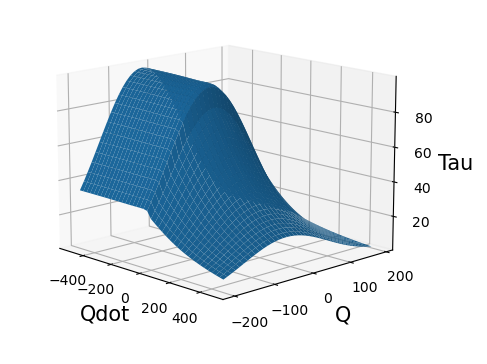
\includegraphics[width=\columnwidth]{figures/graph_force_vitesse_longueur.png}\\
\caption{Surface representing the nonlinear constraint for torque/position/velocity relationship}
\label{fig:graph_force_vitesse_longueur}
\end{figure}

To accelerate the solving of the problem while using \emph{ipopt}, the problem was first approximately solved using a BFGS hessian approximation for 200 iterations maximum.
Then, the solution was re-optimized, from that solution, with an exact-hessian computations for up to 1000 iterations.

The optimized solution of a \SI{1.28}{\meter} jump height was obtained in \SI{1780}{\second} ($\approx\SI{30}{\minute}$).
The solution reproduced a human proximo-distal strategy, that is activating large segments first (for instance the torso) and adding sequentially the more distal segments, the most distal---and the consequently the last to activate---being the ankle.

